\begin{frame}[fragile]
\begin{columns}
	\column{0.25\textwidth}
	\vskip -0.1cm
	\psset{xunit=0.4cm, yunit=0.4cm}
	\begin{pspicture}(-2,-4.4)(4.4,4.45)%
	\tiny%
	\newcommand{\tangentWidth}{1pt}%
	\newcommand{\tangentColor}{black}%
	\fcAxesStandard{-2}{-4.4}{4.4}{4.4}%
	\pstVerb{%
		40 dict begin /stickingCoeffOne 1.2 def /stickingCoeffTwo -0.2 def  /coeffA 0.2 def /coeffB 1.2 def /theFun {x x x mul mul x coeffA mul coeffB add add sqrt} def%
	}%
	\pstVerb{%
		/xOne -1 def %
		/xTwo 0 def %
    /xFour -1 def %
	}%
\onlyNoH{3-}{\pstVerb{%
	/xOne -0.8 def %
	/xTwo 0 def %
}}%
	\pstVerb{%
		%Input: xA yA xB yB. Let (xA, yA) * (xB, yB) = (xC, yC). 
		%This function outputs xC, and the next function outputs yC.
		/xNew {
			20 dict begin /a coeffA def /b coeffB def
			/yB exch def /xB exch def /yA exch def /xA exch def 
			b 2 1 div mul xA a mul add xB a mul add yB yA mul -2 1 div mul add xB 2 1 div exp xA mul add xB xA 2 1 div exp mul add xB xA mul -2 1 div mul xA 2 1 div exp add xB 2 1 div exp add div
			end
		} def %
		/yNew {
			20 dict begin /a coeffA def /b coeffB def
			/yB exch def /xB exch def /yA exch def /xA exch def 
			yA b mul 2 1 div mul yB b mul -4 1 div mul add b yA mul 2 1 div mul add yA xA mul a mul add yB xA mul a mul -3 1 div mul add yA xB mul a mul add yB xB mul a mul -1 1 div mul add xB a mul yA mul 2 1 div mul add xB 3 1 div exp yA mul 2 1 div mul add yB xA 3 1 div exp mul -1 1 div mul add yA xB 3 1 div exp mul -1 1 div mul add yA xB 2 1 div exp mul xA mul 3 1 div mul add yB xB mul xA 2 1 div exp mul -3 1 div mul add xA 3 1 div exp -1 1 div mul xB 3 1 div exp add xB 2 1 div exp xA mul -3 1 div mul add xB xA 2 1 div exp mul 3 1 div mul add div
			end
		} def %
		/yOne  1 dict begin /x xOne def theFun end def%
		/yTwo  1 dict begin /x xTwo def theFun end def%
		/yFour 1 dict begin /x xFour def theFun -1 mul end def%
	}%
	\psplot[linecolor=\fcColorGraph, plotpoints = 300]{-1}{2.5}{theFun}%
	\psplot[linecolor=\fcColorGraph, plotpoints = 300]{-1}{2.5}{theFun -1 mul}%
	\pstVerb{%
		/xThree xOne yOne xTwo yTwo xNew def%
		/yThree xOne yOne xTwo yTwo yNew def%
    /xFive xThree yThree xFour yFour xNew def%
    /yFive xThree yThree xFour yFour yNew def%
    /xSix xTwo yTwo xFour yFour xNew def%
    /ySix xTwo yTwo xFour yFour yNew def%
	}%
\newcommand{\secant}{%
	\psline[linewidth=\tangentWidth, linecolor=\tangentColor](!%
	\pointOneX\space stickingCoeffOne mul \pointTwoX\space stickingCoeffTwo mul add %
	\pointOneY\space stickingCoeffOne mul \pointTwoY\space -1 mul stickingCoeffTwo mul add %
	)(!%
	\pointOneX\space stickingCoeffTwo mul \pointTwoX\space stickingCoeffOne mul add %
	\pointOneY\space stickingCoeffTwo mul \pointTwoY\space -1 mul stickingCoeffOne mul add %
	)%
}%
\newcommand{\doublePerpendicular}{%
	\fcPerpendicular[linestyle=dotted]{[\pointTwoX\space \pointTwoY\space -1 mul]}{[-1 0]}{0.12}%
	\psline[linestyle=dotted](! \pointTwoX\space \pointTwoY\space)(! \pointTwoX\space 0)%
	\fcFullDot[linecolor=green]{\pointTwoX\space}{\pointTwoY\space -1 mul}%
}%
\uncover<1,5->{%
	\rput[tl](! xThree yThree -1 mul){$C'$}%
	\fcFullDot{xThree}{yThree}%
\newcommand{\pointOneX}{xOne}%
\newcommand{\pointOneY}{yOne}%
\newcommand{\pointTwoX}{xThree}%
\newcommand{\pointTwoY}{yThree}%
  \secant%
\doublePerpendicular%
	\rput[bl](! xThree yThree){$\alertNoH{9}{C}$}%
}%
\onlyNoH{5}{%
	\fcFullDot[linecolor=blue]{xThree}{yThree}%
}%
\uncover<6->{%
\renewcommand{\pointOneX}{xThree}%
\renewcommand{\pointOneY}{yThree}%
\renewcommand{\pointTwoX}{xFour}%
\renewcommand{\pointTwoY}{yFour -1 mul}%
\secant%
\renewcommand{\pointOneX}{xThree}%
\renewcommand{\pointOneY}{yThree}%
\renewcommand{\pointTwoX}{xFive}%
\renewcommand{\pointTwoY}{yFive}%
\doublePerpendicular%
\fcFullDot[linecolor=red]{xFive}{yFive}%
\rput[t](! xFive yFive -0.15 add){$E$}
}%
\uncover<7->{%
\renewcommand{\pointOneX}{xTwo}%
\renewcommand{\pointOneY}{yTwo}%
\renewcommand{\pointTwoX}{xSix}%
\renewcommand{\pointTwoY}{ySix}%
\secant%
\doublePerpendicular%
\fcFullDot[linecolor=red]{xSix}{ySix}%
\onlyNoH{7}{%
\fcFullDot[linecolor=blue]{xSix}{ySix}%
}%
\rput[tr](! xSix ySix -0.15 add){$\alertNoH{9}{F}$}
}%
\uncover<8->{%
\pstVerb{/stickingCoeffOne 1.1 def /stickingCoeffTwo -0.1 def %
}%
\renewcommand{\pointOneX}{xOne}%
\renewcommand{\pointOneY}{yOne}%
\renewcommand{\pointTwoX}{xSix}%
\renewcommand{\pointTwoY}{ySix -1 mul}%
\secant%
\renewcommand{\pointTwoY}{ySix}%
\doublePerpendicular%
}%
\onlyNoH{6,8}{\fcFullDot[linecolor=blue]{xFive}{yFive}}%
	\fcFullDot{xOne}{yOne}%
	\fcFullDot{xTwo}{yTwo}%
\uncover<4->{%
  \fcFullDot{xFour}{yFour}%
\onlyNoH{4}{%
  \fcFullDot[linecolor=blue]{xFour}{yFour}%
}%
\rput[t](! xFour yFour -0.15 add){$\alertNoH{9}{D}$}%
}%
\renewcommand{\tangentColor}{pink}%
\renewcommand{\tangentWidth}{1.5pt}%
\onlyNoH{9}{%
\renewcommand{\pointTwoY}{ySix -1 mul}
\secant%
\renewcommand{\pointOneX}{xThree}%
\renewcommand{\pointOneY}{yThree}%
\renewcommand{\pointTwoX}{xFour}%
\renewcommand{\pointTwoY}{yFour -1 mul}%
\secant%
\fcFullDot[linecolor=brown]{xFive}{yFive -1 mul}%
}%
	\rput[tl](! xOne yOne){$\alertNoH{9}{A}$}%
	\rput[br](! xTwo yTwo){$B$}%
	\pstVerb{end}%
	\end{pspicture}
	
	\column{0.75\textwidth}
	\begin{definition}[Elliptic curve group law]
		\begin{itemize}
			\item If line through $A,B$ non-vertical, define $A\cdot B = C$.
			\item Define $A\cdot A$ similarly but use the tangent through $A$ in place of the line through $A, B$.
			\item If line through $A,B$ vertical, define $A\cdot B = \mathbf 1$.
			\item Define $\mathbf 1\cdot A = A\cdot \mathbf 1 = A$ for all $ A$.
		\end{itemize}
	\end{definition}
\end{columns}
\begin{itemize}
\item<2-> $\cdot$ turns the points on the curve into a group.
\item<3-> In particular: why does the associative law hold:

\hfil \hfil $ \underbrace{ \alertNoH{6}{ \left( \underbrace{ \alertNoH{5}{A\cdot B}}_{\alertNoH{5}{=C} } \right) \cdot\alertNoH{4}{ D}} }_{\alertNoH{6}{ =E}} \stackrel{?}{=}  \underbrace{\alertNoH{8}{ A\cdot \left( \underbrace{ \alertNoH{7}{B\cdot D}}_{\alertNoH{7}{=F}}\right) } }_{\alertNoH{8}{=E}}$
\item<9-> I.e., why does  $\alertNoH{9}{AF}$ intersect $\alertNoH{9}{DC}$ on a \alertNoH{9}{point on the curve}?
\item<10-> When we derive formulas, for graphical construction, we can algebraically prove the above.
\item<11-> However our proof will appear an algebraic coincidence/miracle.
\item<12-> An answer to why this all works is beyond current scope.
\end{itemize}



\vskip 10cm

\end{frame}

\begin{frame}
\begin{columns}[T]
\column{0.5\textwidth}
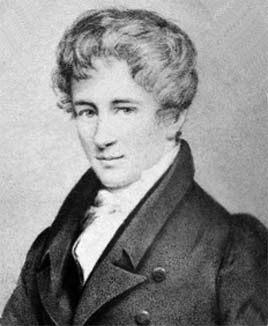
\includegraphics[height=5cm]{\freecalcBaseFolder/modules/crypto-digital-signature-algorithm/images/NielsHenrikAbel.jpg}

Niels Henrik Abel (1802-1829), pioneer of modern algebra and elliptic functions. Abelian groups are named after him.
\column{0.5\textwidth}
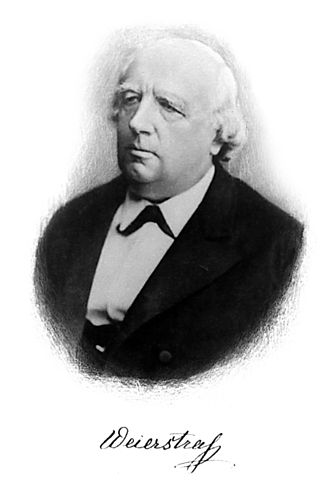
\includegraphics[height=5cm]{\freecalcBaseFolder/modules/crypto-digital-signature-algorithm/images/KarlWeierstrass.jpg}

Karl Weierstrass (1815-1897), pioneer of elliptic functions. The definition of elliptic curve given in our text is sometimes called ``Weierstrass normal form''.

\end{columns}
\end{frame}